\chapter{PPPoE, GRE, eBGP}

\section{PPPoE}

Ethernet links do not natively support PPP. A solution to this problem is PPP over Ethernet (PPPoE). PPPoE creates a PPP tunnel over an Ethernet connection. This allows PPP frames to be sent across the Ethernet cable to the ISP from the customer’s router.\\

To create a PPP tunnel, the configuration uses a \emph{dialer interface}. A dialer interface is a virtual interface. The PPP configuration is placed on the dialer interface, not the physical interface. 

\begin{verbatim}
interface dialer 1
  encapsulation ppp
  ip address negotiated
\end{verbatim}

The PPP CHAP is then configured with hostname Cust1 and password cisco123.
 
\begin{verbatim}
interface dialer 1
  ppp authentication chap callin
  ppp chap host name Cust1
  ppp chap password cisco123
\end{verbatim}

Dialer interface is linked to the Ethernet interface with the \verb|dialer pool| command. Remember to set MTU to 1492 to accommodate PPPoE headers.

\begin{verbatim}
interface dialer 1
  dialer pool 1
  mtu 1492
  no shutdown
\end{verbatim}

The physical Ethernet interface g0/1 with PPPoE is enabled with the command \verb|pppoe enable| interface configuration command. Then it is linked to the Dialer interface with the \verb|pppoe-client dial-pool-number <number>| interface configuration command.

\begin{verbatim}
interface g0/1
  no ip address
  pppoe enable
  pppoe-client dial-pool-number 1
\end{verbatim}

Finally, use the following commands to verify PPPoE:

\begin{verbatim}
show ip int brief
show int dialer 1
show ip route
show pppoe session
debug ppp {negotiation | authentication | events}
\end{verbatim}

\section{GRE}

\subsection{Introduction}

GRE, IPsec, web-based SSL are the three methods of establishing a VPN connection offered by Cisco devices. GRE is a out-dated, non-secure, stateless, site-to-site VPN tunneling protocol. GRE supports the encapsulation of \textbf{any OSI Layer 3 protocol} and \textbf{47} is used in the protocol field in IP header (figure \ref{GREpacket}). GRE also supports multiprotocol and IP multicast tunneling.\\

GRE is the default tunnel interface mode for Cisco IOS software. GRE does not provide encryption or any other security mechanisms. Therefore, data that is sent across a GRE tunnel is not secure.\\

\begin{figure}[hbtp]
\caption{Header for GRE encapsulated packet header}\label{GREpacket}
\centering
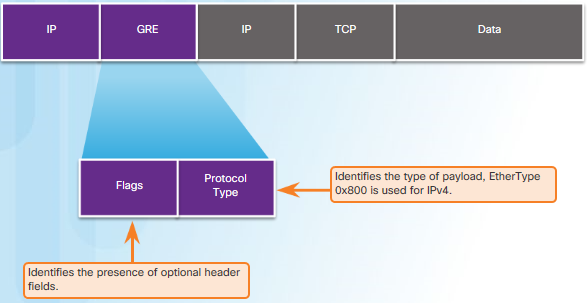
\includegraphics[scale=1]{pictures/GREpacket.PNG}
\end{figure}

Three circumstances can cause a GRE tunnel to be in an up/down state:
\begin{itemize}
\item The tunnel interface is down.
\item A valid route to the destination address is missing from the routing table.
\item The tunnel address is routed through the tunnel itself.
\end{itemize}

\subsection{Configuration}

Five steps to configuring a GRE tunnel (figure \ref{GREexample}):

\begin{figure}[hbtp]
\caption{Configure GRE VPN tunnel}\label{GREexample}
\centering
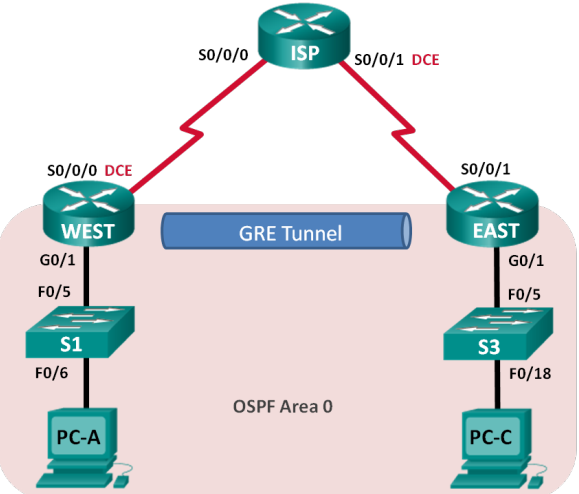
\includegraphics[scale=0.5]{pictures/GREexample.PNG}
\end{figure}

\begin{enumerate}
\item \textbf{Create a tunnel interface:} \\

Configure the tunnel interface on the WEST router. Use s0/0/0 as the tunnel source interface and 10.2.2.1 (IP address of EAST router s0/0/1) as the tunnel destination.

\begin{verbatim}
WEST(config)# interface tunnel 0
WEST(config-if)# ip address 172.16.12.1 255.255.255.252
WEST(config-if)# tunnel source s0/0/0
WEST(config-if)# tunnel destination 10.2.2.1
\end{verbatim}

Configure the tunnel interface on the EAST router. Use s0/0/1 as the tunnel source interface and 10.1.1.1 (IP address of WEST router s0/0/0) as the tunnel destination.

\begin{verbatim}
EAST(config)# interface tunnel 0
EAST(config-if)# ip address 172.16.12.2 255.255.255.252
EAST(config-if)# tunnel source 10.2.2.1
EAST(config-if)# tunnel destination 10.1.1.1
\end{verbatim}

\item \textbf{Verify that the GRE tunnel is functional:} Verify the status of the tunnel interface on the WEST and EAST routers using \verb|show interface tunnel 0| and \verb|show ip interface brief| commands.

\item \textbf{Enable routing over the GRE Tunnel:} After the GRE tunnel is set up, the routing protocol can be implemented. For GRE tunneling, a network statement will include the \underline{IP network of the tunnel}, instead of the network associated with the serial interface. Remember that the ISP router is not participating in this routing process.

\begin{verbatim}
WEST(config)# router ospf 1
WEST(config-router)# network 172.16.12.0 0.0.0.3 area 0

EAST(config)# router ospf 1
EAST(config-router)# network 172.16.12.0 0.0.0.3 area 0
\end{verbatim}

If BGP is used instead of OSPF or EIGRP, the neighbor statement will include the \underline{IP network of the tunnel}, instead of the network associated with the serial interface.

\begin{verbatim}
WEST(config)# router bgp 65000 
WEST(config-router)# neighbor 172.16.12.2 remote-as 65001

EAST(config)# router bgp 65001
EAST(config-router)# neighbor 172.16.12.1 remote-as 65000
\end{verbatim}

\end{enumerate}

\section{eBGP}

\subsection{Introduction}

Border Gateway Protocol (BGP) is an Exterior Gateway Protocol (EGP). BGP updates are encapsulated over TCP on port \textbf{179}. We use BGP when an autonomous system (AS) has connections to \emph{multiple} ASs (known as multi-homed). BGP should not be used when there is a \emph{single} connection to the Internet or another AS (known as single-homed).\\

There are three common ways an organization can choose to implement BGP in a multi-homed environment: Default Route Only, Default Route and ISP Routes, All Internet Routes (this would include routes to over 550,000 networks).\\

External BGP is the routing protocol used between routers in different autonomous systems. Internal BGP is the routing protocol used between routers in the same AS. Two routers exchanging BGP routing information are known as BGP peers.\\

Internal routing protocols (OSPF, EIGRP, RIP, etc.) use a specific metric (e.g. OSPF’s cost) for determining the best paths to destination networks. BGP does \emph{not} use a \emph{single} metric like IGPs. Instead it uses several \emph{attributes} including a list of AS numbers necessary to reach a destination network. Therefore BGP is known as a \emph{path vector} routing protocol. Also, because of this, a misconfiguration of a BGP router could have negative effects throughout the entire Internet.

\subsection{Configuration}

To implement eBGP for this course, you will need to complete the following tasks:
\begin{enumerate}
\item Enable BGP routing and identify the AS number
\item Configure BGP neighbor(s) (peering).
\item Advertise network(s) originating from this AS.
\end{enumerate}

\begin{verbatim}
R2(config)# router bgp 65000 
R2(config-router)# neighbor 209.165.200.1 remote-as 65001
R2(config-router)# network 198.133.219.0 mask 255.255.255.248 
R2(config-router)# end
R2# show ip route
R2# show ip bgp 
R2# show ip bgp summary
\end{verbatim}

